\documentclass[pdflatex,sn-mathphys-num]{sn-jnl}% Math and Physical Sciences Numbered

\usepackage{graphicx}
\usepackage{tabularx,booktabs}
\usepackage{amsmath}
\usepackage{xcolor}
\usepackage{enumitem}
\usepackage{fancyhdr}
\usepackage{caption}
\usepackage{textcomp}
\usepackage{listings}
\usepackage{tikz}
\newcommand{\logref}[1]{\textit{(Log File, #1)}}

\usetikzlibrary{positioning,arrows.meta}


\begin{document}

\title[Article Title]{IK-Dron Desarollo}


\author{ \fnm{Gutiérrez C} \sur{José de Jesus}, \fnm{Martínez P} \sur{Luis Guillermo}, \fnm{Mares M} \sur{Julio Cesar}\footnote{Primera Edición 2021}


\fnm{Contreras R} \sur{Orlando},\fnm{ Garcia B} \sur{Iker}\footnote{Segunda Edición 2026}
}

\affil[3]{\orgdiv{Department of Electronic Systems}, \orgname{UAA}, \orgaddress{\street{Av. Universidad 940}, \city{Aguascalientes}, \postcode{20131}, \state{Aguascalientes}, \country{México}}}

%%==================================%%
%% Sample for unstructured abstract %%
%%==================================%%

\abstract{Hoy en día existe una extensa variedad de drones, hay de diferentes tipos: de aire, agua y tierra. En este documento nos enfocaremos en el desarrollo de un drone aéreo para carreras, veremos las piezas que lo componen, cuáles son las opciones y cuál sería la mejor para tener un desempeño eficiente y posteriormente veremos si es rentable realizarlo o es mejor adquirir un drone ya construido.}


%% me dices si ocupas ayuda con algo ire a desyunar oki probecho mevaleverga
%%================================%%
%% Sample for structured abstract %%
%%================================%%

\keywords{Drone, Control PID, Control de velocidad.}

%%\pacs[JEL Classification]{D8, H51}

%%\pacs[MSC Classification]{35A01, 65L10, 65L12, 65L20, 65L70}

\maketitle

\newpage
\tableofcontents
\newpage
\section{Marco Teórico}

El primer drone del que se tiene constancia data del año 1922 y lo construyó George de Bothezat, a pesar de que no consiguió levantarlo a más de cinco metros del suelo.

Estas aeronaves sin tripulación humana están compuestas por varios componentes, que describimos a continuación:

\subsection{Motores con su propela}

Los motores para drones son motores eléctricos, de acuerdo, pero han sido diseñados para una aplicación tan específica que tienen algunas características muy particulares. Hay tantas variables que afectan el comportamiento de un motor que todo puede llegar a ser muy controvertido y complicado.

Las principales características de un motor para drone son las siguientes:

\subsubsection{Ratio empuje/peso}

Cuando el drone está completamente armado se tiene que considerar el peso del mismo, entonces, la combinación de motor con propela debería dar un empuje mínimo el doble del peso del drone, para que pueda levantarlo. Por ejemplo, si tenemos un drone que pesa 2 kg el empuje debería ser mínimo de 4 kg.

Como se mencionó esto depende de la combinación motor propela. El ratio comúnmente se mide así: 5:1, lo que significa que es 5 veces el peso del drone, si se quiere que el drone sea rápido se puede optar por un ratio de 8:1 a 10:1.

\subsubsection{Número de electroimanes e imanes permanentes}

Comúnmente se usan motores sin escobillas y comúnmente el tamaño se define por 4 dígitos. Un ejemplo sería un motor AABB, donde AA, que son los primeros dígitos representan el diámetro del estator y los últimos dígitos, BB, la altura del rotor. El tamaño del motor tiene dos características, las cuales son:
\begin{itemize}
    \item Entre más alto sea el estator, mayor RPM tendrá el motor
    \item Cuanto mayor diámetro tenga el estator, mayor par generado a menos RPM
\end{itemize}

\subsubsection{KV Constante de velocidad}

Esto tal vez sea una de las partes más importantes de ver a la hora de escoger un motor, la constante de velocidad significa: \textit{RPM por cada volt}. Entonces por ejemplo si se tiene un motor con 2000 KV y se tiene una batería LiPo de 12 V, el motor girará a 24000 RPM.

Entonces si se tienen propelas muy grandes lo ideal sería escoger un motor con bajo KV, ya que los motores con bajo KV generan más par motor, en cambio un motor con un gran KV no ocuparía unas hélices tan grandes, ya que genera más RPM.

\subsubsection{Tamaño del motor}

Probablemente a la hora de escoger un motor tengan escrito algo como esto: ``1806'' o ``1105'', etc. Esto hace alusión al tamaño del motor. Los primeros dos dígitos te dicen la longitud del motor, y los últimos dos dígitos te dicen la altura del motor.

También puede haber casos en los que te encuentres datos como: ``12N14P'', esto hace alusión al número de electroimanes e imanes permanentes que tiene el motor. Los dígitos antes de la letra ``N'', son los electroimanes que tiene el motor, y los números después de la letra ``N'' y antes de la letra ``P'', son los imanes permanentes, esto no tiene mucha importancia ya que comúnmente todos los motores tienen la siguiente configuración ``12N14P''.

\subsubsection{Tamaño del chasis}

Lo que primero se debe escoger para armar un drone es el chasis ya que, dependiendo del tamaño de este, se puede estimar más o menos el tamaño de las hélices y en consecuencia el KV del motor. Por lo que a continuación se muestra una tabla dependiendo del tamaño del chasis, para escoger hélices y motores.

\begin{table}[!h]
\centering
\caption{Tabla de guía para escoger un motor y su propela}
\label{tab:motor_guide}
\begin{tabular}{|c|c|c|c|}
\hline
\textbf{Tamaño del chasis} & \textbf{Tamaño de Hélices} & \textbf{Tamaño del Motor} & \textbf{KV} \\
\hline
150 mm o menor & 3'' o menor & 1105-1306 o menor & 3000 KV o más \\
\hline
180 mm & 4'' & 1806 & 2600 KV - 3000 KV \\
\hline
210 mm & 5'' & 2204-2208, 2306 & 2300 KV-2600 KV \\
\hline
250 mm & 6'' & 2204-2208, 2306 & 2000 KV-2300 KV \\
\hline
350 mm & 7'' & 2208 & 1600 KV \\
\hline
450 mm & 8'', 9'', 10'' o mayor & 2212 o mayor & 1000 KV o menos \\
\hline
\end{tabular}
\end{table}

Entonces por ejemplo si se compró un chasis de 180 mm, lo ideal sería comprar una hélice de tamaño 4'', un motor de tamaño 1806 con un KV entre 2600 KV y 3000 KV.

\subsubsection{Eficiencia del motor}

Este factor es muy importante ya que nos determina si estamos consumiendo energía innecesaria y por esto nuestra batería se consume más rápido, o consumimos la energía necesaria para que vuele el drone.

Este dato no te lo da el fabricante, ya que depende de la batería y los ESC que uses. Esto se calcula así:

\begin{equation}
\mathrm{Eficiencia} = \frac{\mathrm{Empuje}}{\mathrm{Voltaje} \times \mathrm{Corriente}} = \frac{\mathrm{Ratio}}{\mathrm{Potencia}}
\end{equation}

Entre mayor sea este número, mayor será la eficiencia del motor.

\vspace{0.5em}

A continuación, se mostrará un ejemplo de un motor con sus especificaciones, de las cuales nos debería 
importar más, el tamaño del motor, la KV, el empuje y el peso. Aunque las otras características pueden ser 
muy útiles para un excelente diseño. 
\begin{figure}[!h]
    \centering
    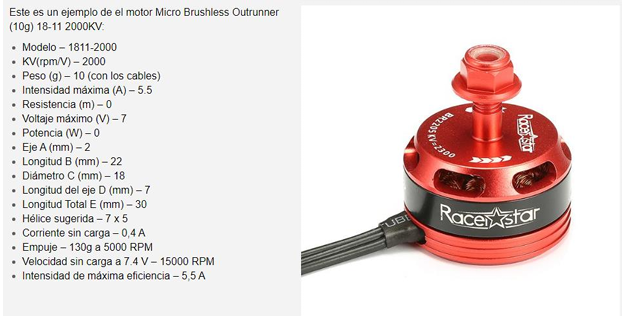
\includegraphics[width=0.5\linewidth]{src/EjemploMotor.png}
    \caption{ Ejemplo de un motor para drone con sus especificacione}
    \label{fig:placeholder}
\end{figure}

\subsection{Controladores de velocidad (ESC)}

El ESC o variador es un componente esencial dentro de un drone, por sus siglas (Electronic Speed Controller) nos encontramos ante un controlador de velocidad electrónico. Un sistema capaz de definir la velocidad de giro de un motor brushless mediante la generación de pulsos compatibles con este tipo de motores.

Se componen de varios cables, de entrada tiene dos cables, los cuales corresponden a la entrada de alimentación de la batería. También cuentan con otros tres cables, normalmente van juntos, se conectan al motor para proveerlo de alimentación mediante pulsos, también tienen un conector con dos o tres cables trenzados, dicho conector va conectado a la controladora, de la que recibe los datos para mover el motor.

\begin{figure}[!h]
    \centering
    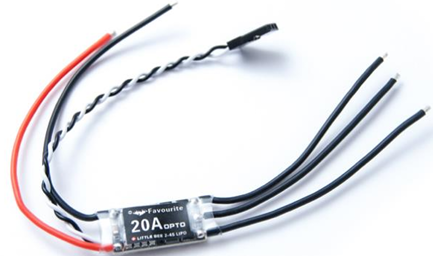
\includegraphics[width=0.5\linewidth]{src/ESC.png}
    \caption{Ejemplo de controlador de velocidad.}
    \label{fig:placeholder}
\end{figure}
\subsubsection{Funcionamiento de un ESC}

Supongamos que un piloto mueve el Stick de aceleración a fondo, la controladora enviará los datos calculados en función de la posición del drone y de la posición del stick. La información en forma de datos viajará a través del conector correspondiente hacia el ESC, en este momento el variador demandará la energía necesaria a la batería a través de sus cables de conexión, luego de esto se produce la traducción a pulsos dentro del ESC, y se transmite al motor a través de tres conectores.

\subsection{Batería}

Las baterías son un componente esencial en el diseño de drones, ya que proporcionan la energía necesaria para alimentar los motores, controladores y otros sistemas electrónicos. La selección de la batería adecuada es crucial para garantizar un rendimiento óptimo y una mayor duración del vuelo. Las baterías más comunes utilizadas en drones son las de polímero de litio (LiPo), debido a su alta densidad energética, bajo peso y capacidad de descarga rápida, siendo un tipo de batería que se usa en diversos dispositivos electrónicos.


Al elegir una batería, es importante considerar factores como la capacidad (medida en mAh), el voltaje (medido en V) y la tasa de descarga (medida en C) para asegurarse de que se adapte a las necesidades específicas del dron y sus componentes.


\begin{figure}[!h]
    \centering
    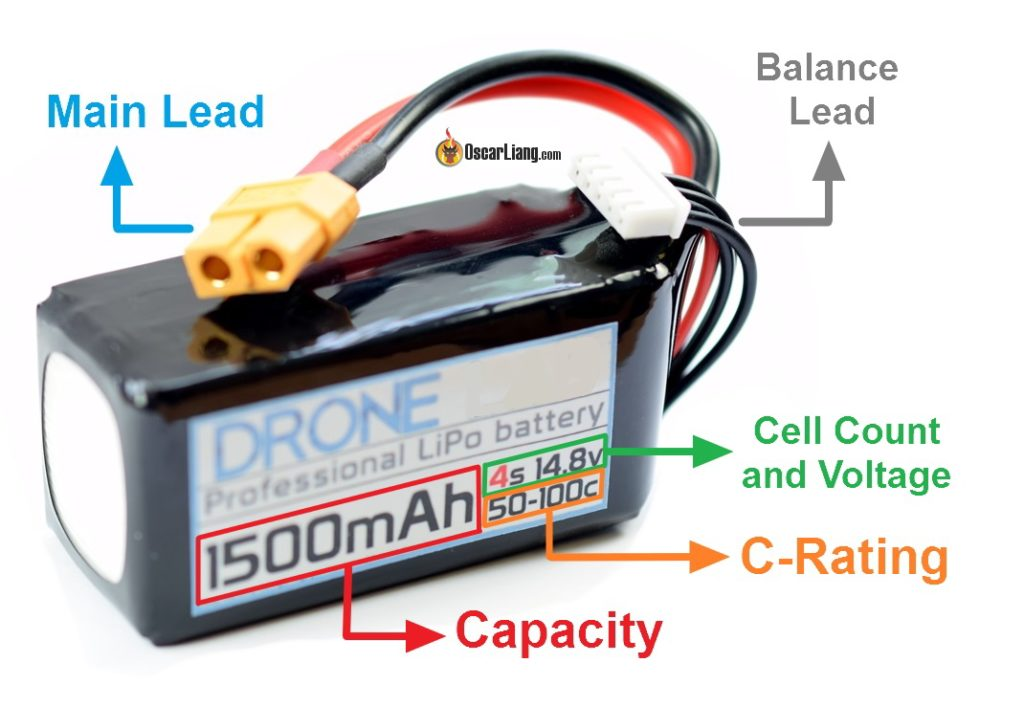
\includegraphics[width=0.65\linewidth]{src/Bateria.png}
    \caption{Caracteristicas de la bateria}
    \label{fig:placeholder}
\end{figure}


Las principales características de una batería LiPo son las siguientes:
\subsubsection{Capacidad}

La capacidad de la batería, medida en miliamperios hora (mAh), indica la cantidad de carga eléctrica que la batería puede almacenar. Una mayor capacidad generalmente se traduce en un tiempo de vuelo más largo, pero también puede aumentar el peso de la batería, lo que afecta la maniobrabilidad del dron. Es importante encontrar un equilibrio entre la capacidad de la batería y el peso para optimizar el rendimiento del dron.
Por practicidad se utilizará la notación de capacidad en Ah (amperios hora) en lugar de mAh, esto se hace para facilitar los cálculos relacionados con la tasa de descarga y la corriente que la batería puede suministrar. Por ejemplo, una batería de 2000 mAh se expresaría como 2 Ah, lo que simplifica la comprensión de la capacidad y su relación con otros parámetros como la tasa de descarga (C) y la corriente máxima que puede suministrar.
\cite{rogerlipo}
%https://www.rogershobbycenter.com/lipoguide

\subsubsection{Voltaje de la batería y cuenta de celdas S}

Las celdas de Li-Po es de 3.7V (1 cell = 1S), por lo que una batería de 4S (4 celdas en serie) tendrá un voltaje nominal de 14.8V (3.7V x 4). Pueden haber los siguientes paquetes de baterías, el voltaje es algo fundamental en motores ya que determina la potencia que estos pueden generar, a mayor voltaje mayor potencia, sin embargo también se debe considerar la capacidad de la batería y la tasa de descarga para asegurarse de que el sistema funcione de manera eficiente y segura.
\cite{gensacelipo}
% https://gensace.de/pages/lipo-battery-guide
\begin{itemize}
\item 3.7V battery = 1 cell x 3.7V= 1S battery
\item 7.4V battery = 2 cells x 3.7V= 2S battery
\item 11.1V battery = 3 cells x 3.7V= 3S battery
\item 14.8V battery = 4 cells x 3.7V= 4S battery
\item 18.5V battery = 5 cells x 3.7V= 5S battery
\item 22.2 V battery = 6 cells x 3.7V= 6S battery
\item 29.6 V battery = 8 cells x 3.7V= 8S battery
\item 37.0V battery = 10 cells x 3.7V= 10S battery
\item 44.4V battery = 12 cells x 3.7V= 12S battery
\end{itemize}


\subsubsection{C rating o velocidad de descarga}
La taza de descarga (C) es una factor de que tan rapido se puede descargar una bateria de forma segura

Las baterias con una mayor taza de descarga tienden a ser mas pesadas y grandes para la misma capacidad, esto es un aspecto interesante a la hora de realizar un diseño de dron, ya que se debe encontrar un equilibrio entre la capacidad de la batería, su peso y su tasa de descarga para optimizar el rendimiento del dron.
\cite{oscarlipo}
% https://oscarliang.com/lipo-battery-guide/

La taza de descarga implica que tanta bateria puede ser drenada de forma segura siendo un factor de la capacidad energetica es decir, si se tiene una bateria de 1Ah con una tasa de descarga de 20C, esto significa que la bateria puede suministrar hasta 20 veces su capacidad en corriente, lo que equivale a 20 x 1Ah = 20A de corriente máxima de descarga continua sin dañar la batería. 
\cite{rclipo}
% https://www.rcteam.com/en/blogs/the-rc-model-blog/lipo-battery-guide
\subsubsection{Conectores}
Una buena batería de Li-Po debe venir acompañado de un buen conector, es algo crucial para que pueda entregar la carga de forma eficiente ya que el conector puede presentar cierta resistencia. Para ello hay que ver los diferentes conectores que existen, como se puede ver en la imagen capturada de \cite{rogerlipo}.
Existen diferentes tipos de conectores, a continuación se dará una breve descripción de cada uno
\begin{figure}[!h]
    \centering
    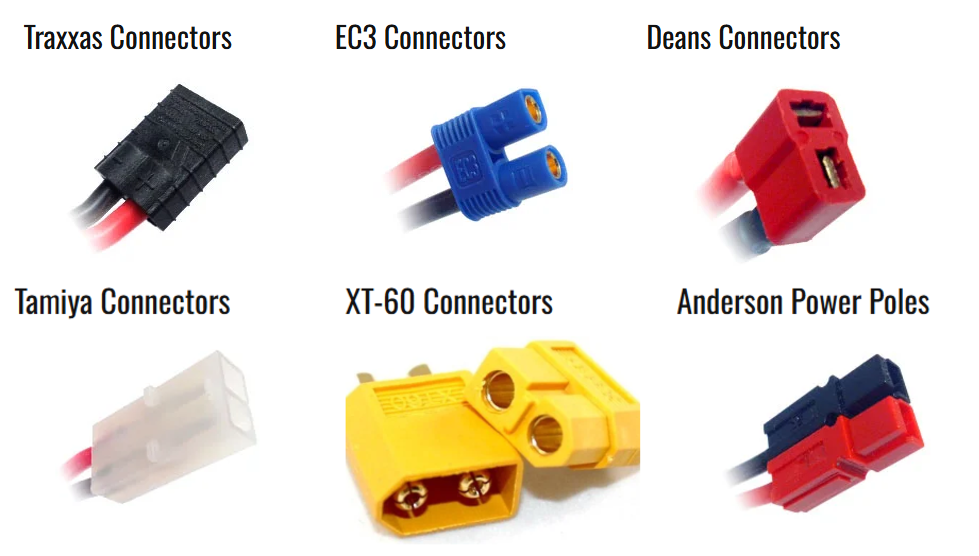
\includegraphics[width=0.5\linewidth]{src/Conectores.png}
    \caption{Tipos de conectores}
    \label{fig:placeholder}
\end{figure}
\begin{itemize}
    \item \textbf{Traxxas:} \\
    Son comunes en carros RC, no requieren un disipador, no hay forma de conectarlo del revés.
    \item \textbf{EC3:} \\
    
    \item \textbf{Dean:} \\ 
    Son algo complicado de soldar, no hay forma de conectarlo del revés, son muy populares en drones de carreras.
    \item \textbf{Tamiya:} \\
    Es un conector terrible que tiene mucha resistencia
    \item \textbf{XT60:} \\
    \item \textbf{Anderson:}\\
    Es un conector de forma curiosa ya que no es macho ni hembra, por lo que puedes conectarlo de cualquier forma, es un conector muy raro de encontrar en el mundo de RC.

\end{itemize}

\subsection{Controladora de vuelo}

El controlador de vuelo es una tarjeta integrada que viene a ser el cerebro del drone. El FC (Flight Controller) contiene un microcontrolador que interpreta las señales recibidas por el receptor de radio (RX) y emite las señales adecuadas a los controladores electrónicos de velocidad de los motores (ESCs) para que el drone vuele cómo y dónde nosotros queramos.

El controlador de vuelo también es donde se conectan todos los sensores (giroscopios, acelerómetros, GPS, barómetro, magnetómetro, sonar, etc.) y todos los periféricos de salida (telemetría, caja negra, buzzer, LEDs, OSD, servos, etc.) que puede llevar el aparato.

Los controladores de vuelo más modernos tienen cada vez más puertas serie para conectar un número mayor de dispositivos, porque la tendencia hoy es claramente centralizar el control de todos los dispositivos que pueda llevar el aparato a través del FC, así pues, hoy se pueden incluso encontrar cámaras HD que permiten su manejo por medio de radiocontrol.

Los FC para cuadracópteros están evolucionando rápidamente: cada vez son más pequeños, usan mejores procesadores y hardware y tienen más y más funciones integradas.

\begin{figure}[!h]
    \centering
    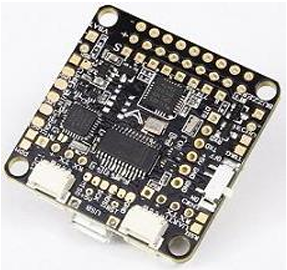
\includegraphics[width=0.5\linewidth]{src/FC.png}
    \caption{Controladora de Vuelo}
    \label{fig:placeholder}
\end{figure}
\subsection{Módulo de distribución de energía}

Estos módulos ayudan a que llegue la energía a cada una de las controladoras de vuelo, también cuentan con reguladores el cual reduce el voltaje hasta 5 V para poder conectar otros módulos de bajo voltaje. Este módulo no cuenta con filtros ni componentes que afecten al voltaje que llegará a los motores, por lo que la principal utilidad de este módulo es tener un cableado más estético.

\begin{figure}[!h]
    \centering
    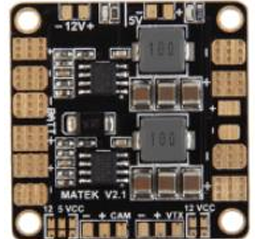
\includegraphics[width=0.5\linewidth]{src/ModuloDistribucion.png}
    \caption{Placa distribuidora de voltaje}
    \label{fig:placeholder}
\end{figure}
\subsection{Transmisor y transceptor}

El transmisor y el receptor son una parte fundamental del drone, porque es con estos dos componentes es con lo que se logra pilotar el vehículo no tripulado, por lo que una mala comunicación entre estos dos podría llegar a causar un accidente o la destrucción de este.

El transmisor debe contar con un mínimo de 4 canales que son: stick derecho eje X y Y, stick izquierdo eje X y Y. Los transmisores normalmente cuentan con 5 o 6 canales, estos canales extra sirven para cambiar el modo de vuelo por si se quiere cambiar la configuración de los sticks.

El transceptor solo puede funcionar con su misma marca de transmisor, aunque existen tarjetas para poder lograr la comunicación universal, aunque esto no es lo ideal. Algunos transceptores son capaces de transmitir telemetría (monitoreo de datos del drone en tiempo real), algunos otros son más ligeros y algunos ofrecen una mejor comunicación, por lo que la elección del transmisor determinará el transceptor.

\begin{figure}[!h]
    \centering
    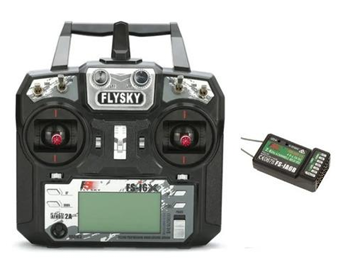
\includegraphics[width=0.5\linewidth]{src/Control.png}
    \caption{Transmisor y receptor de 6 canales}
    \label{fig:placeholder}
\end{figure}
\subsection{Estructura}

La estructura es la parte que define cuantos motores tendrá, el tamaño de las propelas, el peso mínimo y la robustez que tendrá el drone. Esta es la parte donde se montan y se mantienen el resto de los componentes. La función principal es reducir al máximo las vibraciones producidas por los motores al hacer girar las hélices.

Existen estructuras de todo tipo de material como el aluminio, plástico, fibra de vidrio y fibra de carbono. Dependiendo del material del cual esté compuesta la estructura será el peso y la rigidez que tendrá el drone, una estructura muy ligera podría dificultar el vuelo debido al aire que podría circular por la zona.

Hay distintos tipos de configuraciones para las estructuras, la mayor diferencia entre cada configuración es el número de motores que puede llegar a poseer.

\begin{figure}[!h]
    \centering
    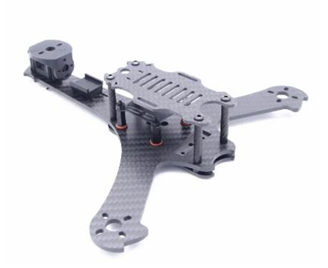
\includegraphics[width=0.5\linewidth]{src/Estructura.png}
    \caption{Estructura de un drone tricoptero}
    \label{fig:placeholder}
\end{figure}

\newpage
\section{Desarrollo}

\subsection{Recursos}
\begin{itemize}
    \item Software LibrePilot
    \item 4 motores brushless
    \item 4 controladores de velocidad
    \item 1 controladora de vuelo
    \item 1 estructura de fibra de carbono
    \item 1 juego de propelas
    \item Control y Receptor
    \item Módulo de distribución de energía
\end{itemize}

\subsection{Procedimiento}

\subsubsection{Comparaciones}

Lo primero que se debe hacer al momento de armar un drone es seleccionar las partes y los componentes de este de acuerdo con tus necesidades, así pues, a continuación se muestran las comparaciones de algunos de los componentes necesarios para un drone.

\paragraph{Motores}

\begin{table}[!h]
\centering
\caption{Comparación de motores}
\label{tab:motors_comparison}
\begin{tabular}{|c|c|c|c|c|c|}
\hline
\textbf{Modelo} & \textbf{Ratio} & \textbf{Tamaño} & \textbf{KV} & \textbf{Peso(g)} & \textbf{Precio} \\
\hline
FlashHobby BE1806 & 130g a 25590 RPM & 1806 & 2300KV & 18g & \$290.95 MXN \\
\hline
Racerstar BR2205 & 660g a 25530 RPM & 2205 & 2300KV & 28g & \$290.95 MXN \\
\hline
Racerstar BR2204 & 365g a 25530 RPM & 2204 & 2300KV & 25g & \$810.17 MXN \\
\hline
E-R2205 & 600g a 21730 RPM & 2205 & 2300KV & 30.5g & \$519.71 MXN \\
\hline
Sunnysky E-R2205 & 600g a 21421 RPM & 2204 & 2300KV & 27g & \$457.32 MXN \\
\hline
\end{tabular}
\end{table}

Como se muestra en la tabla anterior, tenemos una comparación de algunos motores, los cuales son traídos de la página china ``Banggood''. Para este drone se seleccionó el modelo FlashHobby BE1806 con un precio de 290 pesos mexicanos. Se seleccionó este motor ya que es muy pequeño y para la carcasa que se seleccionó era necesario, además de que está a un muy buen precio, el motor tiene un peso muy accesible. Una parte que podría mejorarse sería el empuje ya que solo carga 130g cuando hay 25590 RPM, pero como es un drone de carreras, no pesa mucho por lo que son perfectos para este proyecto.

\paragraph{ESC}

En general, la selección del ESC dependerá del tipo de empuje que necesitemos en nuestro drone, un factor que está muy relacionado con el tipo de batería utilizado y su configuración de motores y hélices.

Hay una norma que suele funcionar, si utilizamos una batería 3S, con un ESC de 12A será más que suficiente, si utilizamos una batería 4S, es conveniente utilizar un ESC de al menos 20A.

\begin{table}[!h]
\centering
\caption{Comparación entre algunos de los ESC en el mercado}
\label{tab:esc_comparison}
\begin{tabular}{|c|c|c|c|c|}
\hline
\textbf{Modelo} & \textbf{Marca} & \textbf{Amperaje} & \textbf{Peso} & \textbf{Precio} \\
\hline
DSHOT600 & Oneshot & 20A & Desconocido & \$314 MXN \\
\hline
BL20A Mini & Flashhobby & 20A & 7.6g & Descontinuado \\
\hline
F396 & LittleBee & 20A & 6g & \$230 MXN \\
\hline
BLHeli Series ESC & Emax & 20A & 28g & \$293 MXN \\
\hline
Simonk Series & Emax & 20A & 28g & \$303 MXN \\
\hline
\end{tabular}
\end{table}

Seleccionamos el ESC de la marca Flashhobby debido a que este es especialmente para drones de carreras, es muy ligero, el acelerador responde rápidamente, la señal del acelerador es un cable de par trenzado, este reduce la perturbación electromagnética producida en el canal de comunicación, por ende el vuelo es más estable. La frecuencia de actualización máxima de la señal del acelerador es de hasta 500 Hz, y es compatible con todos los controles de vuelo.

\paragraph{Módulo de distribución de energía}

\begin{table}[!h]
\centering
\caption{Comparación entre los distribuidores de energía}
\label{tab:pdb_comparison}
\begin{tabular}{|c|c|c|c|c|}
\hline
\textbf{Modelo} & \textbf{Marca} & \textbf{Voltaje salida} & \textbf{Alimentación} & \textbf{Precio} \\
\hline
AP-XT60 & Matek & 9v - 18v & LiPo 4S (13v - 18v) & \$251 MXN \\
\hline
FCHUB-65 & Matek & 5v - 10v & LiPo 3-6S (9v - 26v) & \$168.27 MXN \\
\hline
V3 PDB & Lantian & 5v - 12v & LiPo 2-6S (9V - 26v) & \$209 MXN \\
\hline
PDB Genérico & -- & 5v - 12v & LiPo 4S (13v - 18v) & \$209.34 MXN \\
\hline
\end{tabular}
\end{table}

Después de analizar cada una de las PDB, llegamos a la conclusión que la mejor opción para el drone que queremos construir es el de la marca Lantian, esto porque posee espacio para 4 salidas de 12 V que serán utilizadas para los motores y otros 2 apartados de 5 V, los cuales se utilizan para el receptor y la cámara, además de que la batería que utilizaremos está en el rango de alimentación y será capaz de alimentar a los motores para que lleguen a su RPM máximo.

\paragraph{Controladora de vuelo}

Para seleccionar la mejor controladora, primero debemos distinguir las diferencias entre cada una de ellas. Uno de los dispositivos más importantes dentro del FC es el microcontrolador, actualmente hay cuatro tipos entre los que elegir: F1, F3, F4 y F7, las velocidades máximas de cada micro se muestran en la Tabla \ref{tab:microcontroller_speeds}.

\begin{table}[!h]
\centering
\caption{Velocidades máximas de cada microcontrolador}
\label{tab:microcontroller_speeds}
\begin{tabular}{|c|c|c|c|}
\hline
\textbf{F1} & \textbf{F3} & \textbf{F4} & \textbf{F7} \\
\hline
72 MHz & 72 MHz & 168 MHz & 216 MHz \\
\hline
\end{tabular}
\end{table}

Otra cosa a tener en cuenta es el número de UART con los que cuenta la FC. Un UART es un puerto serial de hardware que te permite conectar dispositivos externos como un receptor digital (SBUS y Spektrum), el OSD, Telemetría, transpondedor de carrera, control de VTX, etc.

Cada UART tiene 2 pines. TX para transmitir datos y RX para recibirlos. El número de UARTs depende del tipo de microcontrolador y de la placa base en la que está montado. Por ejemplo, los FC con un F1 tienen normalmente dos UART, mientras que los F3 y F4 pueden tener de tres a cinco y un F7 puede tener ocho o más.

Otro elemento esencial para el funcionamiento del drone es el IMU. La Unidad de Medición Inercial (IMU) mide el movimiento y orientación del cuadracóptero.

Hay dos propiedades fundamentales de un sensor IMU en un FC que debemos considerar. La velocidad máxima de muestreo y cómo de susceptible es al ruido, tanto eléctrico como mecánico.

Actualmente el IMU más ampliamente usado es el MPU6000 que soporta una velocidad de muestreo de 8 KHz y es una de las más robustas frente al ruido. El consenso general es evitar las MPU6500 y la MPU9250 que aunque tienen mayor velocidad de muestreo son más sensibles al ruido.

Los protocolos de comunicación que conectan el sensor y al procesador son el i2c y el SPI. El preferido es el SPI, que permite al giroscopio una velocidad de refresco mucho más rápida que el i2c.

Una comparación de algunos sensores IMU utilizados en las diferentes FC se encuentra en la Tabla \ref{tab:imu_comparison}.

\begin{table}[!h]
\centering
\caption{IMUs utilizadas en las tarjetas controladoras de vuelo}
\label{tab:imu_comparison}
\begin{tabular}{|c|c|c|}
\hline
\textbf{IMU} & \textbf{Protocolo de Comunicación (BUS)} & \textbf{Máxima frecuencia de muestreo} \\
\hline
MPU6000 & SPI, i2c & 8K \\
\hline
MPU6050 & i2c & 4K \\
\hline
MPU6500 & SPI, i2c & 32K \\
\hline
MPU9150 & i2c & 4K \\
\hline
MPU9250 & SPI, i2c & 32K \\
\hline
ICM20602 & SPI, i2c & 32K \\
\hline
ICM20689 & SPI, i2c & 32K \\
\hline
\end{tabular}
\end{table}

Otras consideraciones a la hora de elegir un FC son:

\begin{itemize}
    \item \textbf{Regulador de voltaje integrado:} Con un regulador de voltaje integrado en el FC, este puede alimentarse directamente desde la batería LiPo e incluso proporcionar salidas a 5 V y 12 V para otro equipo.
    \item \textbf{PDB integrado:} Cuando el PDB está integrado en el FC como una sola tarjeta, tanto tus ESCs, como tu batería LiPo pueden ser conectadas directamente al FC y no hace falta un PDB adicional.
    \item \textbf{OSD integrado:} Un OSD significa On screen display y sirve para mostrar datos sobre la imagen que recibimos en nuestras gafas, es especialmente útil para ver valores como el tiempo de vuelo, el voltaje de la batería y los mAhs consumidos.
    \item \textbf{VTX integrado:} Un VTX es un sistema que envía la señal de vídeo de la cámara FPV en el drone a un receptor VRX autónomo o integrado en unas gafas FPV.
    \item \textbf{Barómetro / Magnetómetro incluidos:} Estos sensores extras son menos importantes para las carreras de mini quads.
\end{itemize}

Se seleccionó la controladora CC3D, este es un controlador de vuelo potente y asequible que es muy popular para usar principalmente en helicópteros miniquad. La principal razón al adquirir esta es que pensábamos en diseñar nuestra propia controladora de vuelo.

\paragraph{Estructura}

Se decidió analizar solamente las estructuras que tuvieran 4 motores, ya que estos poseen mayor estabilidad que los que tienen 3 y son más aerodinámicos que los que tienen 5 o más.

\begin{table}[!h]
\centering
\caption{Comparación entre los chasis}
\label{tab:chassis_comparison}
\begin{tabular}{|c|c|c|c|c|c|}
\hline
\textbf{Modelo} & \textbf{Material} & \textbf{Peso} & \textbf{Hélice} & \textbf{Distancia ejes} & \textbf{Precio} \\
\hline
GEP-KX5 & Fibra de carbono 3k & 115g & 5 in & 243 mm & \$1577 MXN \\
\hline
F2 Mito GS & Fibra de carbono 3k & 125g & 4 in & 250 mm & \$837 MXN \\
\hline
ZMR250 & Fibra de carbono & 118g & 4 in & 250 mm & \$586 MXN \\
\hline
Martian IV & Fibra de carbono & 118g & 5 in & 220 mm & \$670 MXN \\
\hline
LS-210 & Fibra de carbono 3k & 100g & 5 in & 210 mm & \$586 MXN \\
\hline
\end{tabular}
\end{table}

Después de analizar algunas de las carreras de drones, observamos que durante la carrera se presentan distintos obstáculos que solo los drones con ciertas dimensiones lograban superarlos. Los 2 chasis que cumplían con este requisito son ``Martian IV'' y ``LS-210'' aunque la variación es de 10 mm, decidimos utilizar el chasis LS-210, aparte de que tiene menos peso y contiene fibra de carbono más robusto que el otro, está a un buen precio.

\paragraph{Batería}

\begin{table}[!h]
\centering
\caption{Comparación de baterías LiPo}
\label{tab:battery_comparison}
\begin{tabular}{|c|c|c|c|c|}
\hline
\textbf{Modelo} & \textbf{Capacidad} & \textbf{Celdas} & \textbf{C-Rating} & \textbf{Precio} \\
\hline
Limskey 7.4V & 1500 mAh & 2s & 30C & \$157.69 MXN \\
\hline
PYLRC 7.4V & 1600 mAh & 2s & 30C & \$215.83 MXN \\
\hline
Hobby Hub 11.1V & 2200 mAh & 3s & 40C & \$197.06 MXN \\
\hline
Youme Power 7.4V & 6200 mAh & 2s & 50C & \$623.83 MXN \\
\hline
Turnigy 2.2 & 2200 mAh & 3s & 20C-40C & Descontinuado \\
\hline
\end{tabular}
\end{table}

Como se muestra en la tabla anterior, tenemos una comparación de algunas baterías. La batería que recomendamos a usar sería la Hobby Hub 11.1V, ya que está a un buen precio y ofrece lo mismo que la que nosotros usamos. Las baterías se buscaron en la página china ``AliExpress''.

\subsubsection{Diseño de controladora de vuelo}

Como se mencionó, quisimos ir más allá y queríamos diseñar nuestro propio módulo de controladora de vuelo. Tanto el diseño de un PCB como la programación de la misma.

Primero se seleccionaron los componentes que llevaría la controladora de vuelo, siendo el microcontrolador el principal componente: El microcontrolador usado fue una M4, ``STM32F466RE'', ya que nos resultaba más fácil para programar además de que el precio es muy accesible.

Enseguida se colocaron dos reguladores de voltaje de 3.3 V, ya que el microcontrolador y algunos módulos no se les puede energizar con más de esta cantidad.

Los módulos que usamos fueron: el giroscopio (MPU6050), Sensor de presión (BMP280), y el magnetómetro (QMC5883L). Con estos sensores seremos capaces, mediante un control de motores, controlar la altitud, dirección, orientación y velocidad del drone.

Ya con todos los módulos seleccionados, se realizó el esquemático de la controladora de vuelo. Para esto nos basamos en diseños de otras controladoras de vuelo y en los datasheet de los componentes seleccionados. pero se tiene que tener cuidado ya que las conexiones dependen de los componentes que se seleccionaron, por lo que no solo es copiar y pegar, si no analizar las conexiones que se realizaron y después realizar las conexiones en nuestro propio esquemático. El diseño en el que nos 
basamos es el siguiente
\begin{figure}[!h]
    \centering
    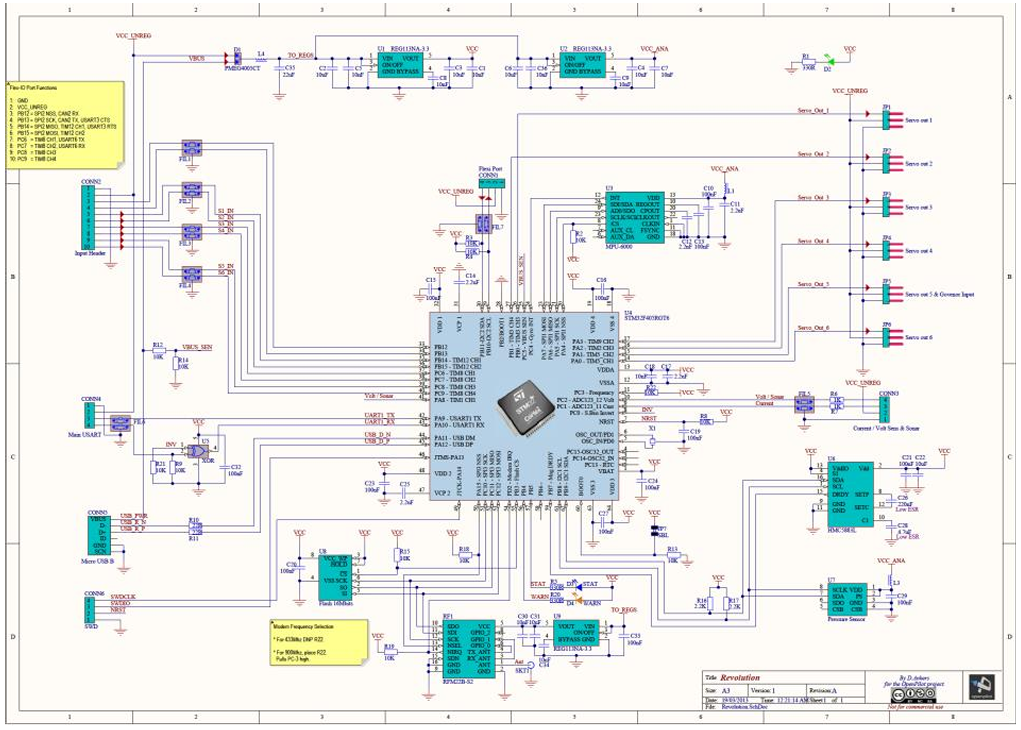
\includegraphics[width=0.5\linewidth]{src/Diseño.png}
    \caption{Esquemático de una controladora de vuelo de un hexacoptero }
    \label{fig:placeholder}
\end{figure}

Seleccionamos los componentes antes mencionados, debido a que también se tiene que ver la 
disponibilidad de ellos en páginas que distribuyan estos componentes. El software seleccionado para 
realizar el esquemático y PCB de la FC es: “EasyEDA”, ya que este software es libre y no necesita de 
una instalación, es una página web con guardado en la nube, con esto más de una persona puede trabajar 
en el diseño, siempre y cuando no trabajen al mismo tiempo. 


“EasyEDA” es una página que es una parte de otra página llamada “LCSC”, que esta nos proporciona 
tanto los componentes, como los PCB. 
Con esto explicado el diseño de nuestro esquemático es el siguiente:

\begin{figure}
    \centering
    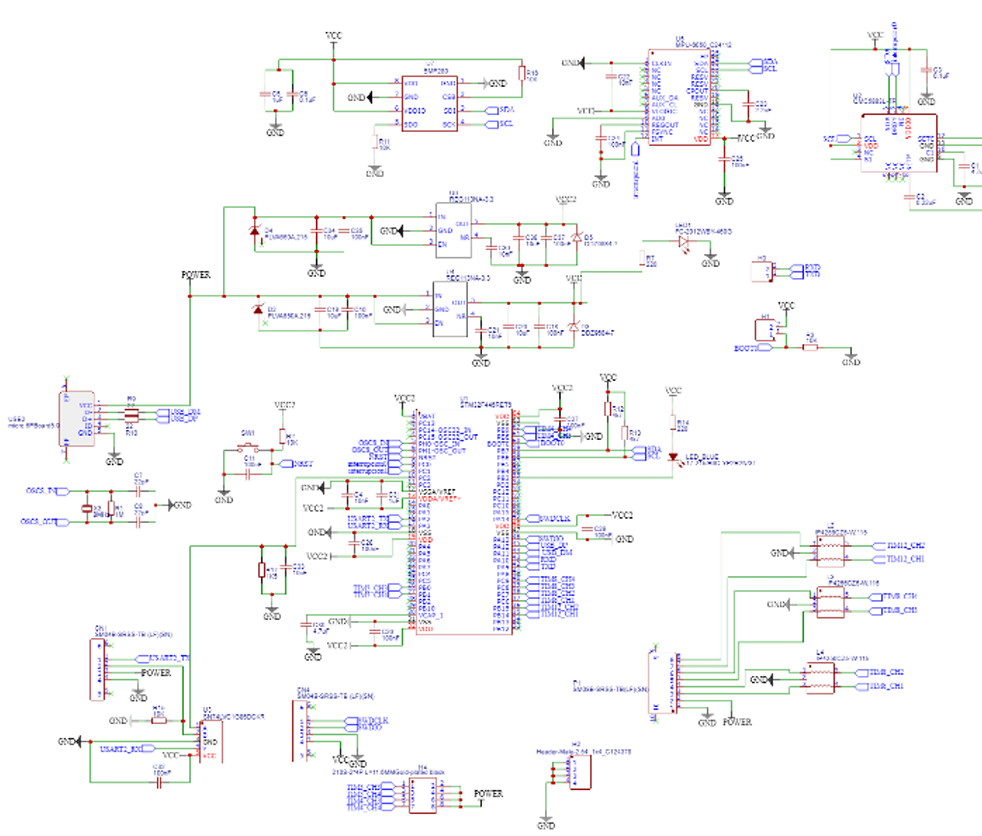
\includegraphics[width=0.5\linewidth]{src/EsquematicoPCB.png}
    \caption{Esquemático de una controladora de vuelo de un quadcoptero }
    \label{fig:placeholder}
\end{figure}

Ahora con el esquemático se realizará el PCB de la FC, para esto es bueno ver protocolos de 
controladoras de vuelo, ya que se busca que el tamaño o las conexiones no sean problemas si esta FC 
se quiere usar para otro tipo de drones, u otros chasis etc. El protocolo usado para la FC es el siguiente:

\begin{figure}
    \centering
    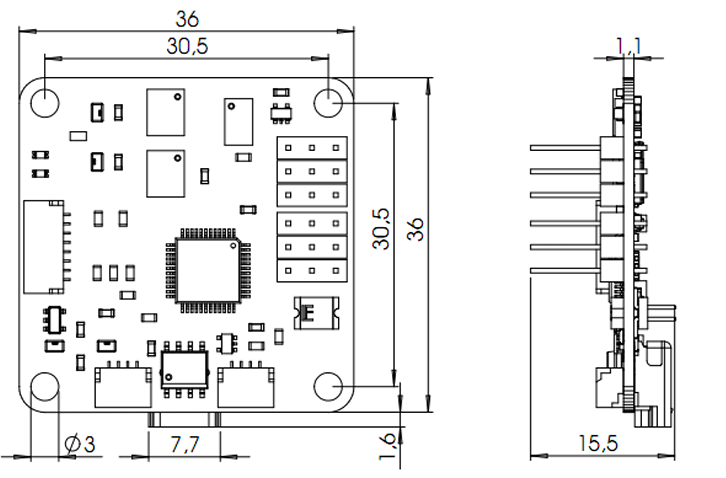
\includegraphics[width=0.5\linewidth]{src/ModeloPCB.png}
    \caption{Protocolo para PCB de una controladora de vuelo}
    \label{fig:placeholder}
\end{figure}


Con este protocolo se realizó el diseño de la FC, el cual es el siguiente: 

\begin{figure}
    \centering
    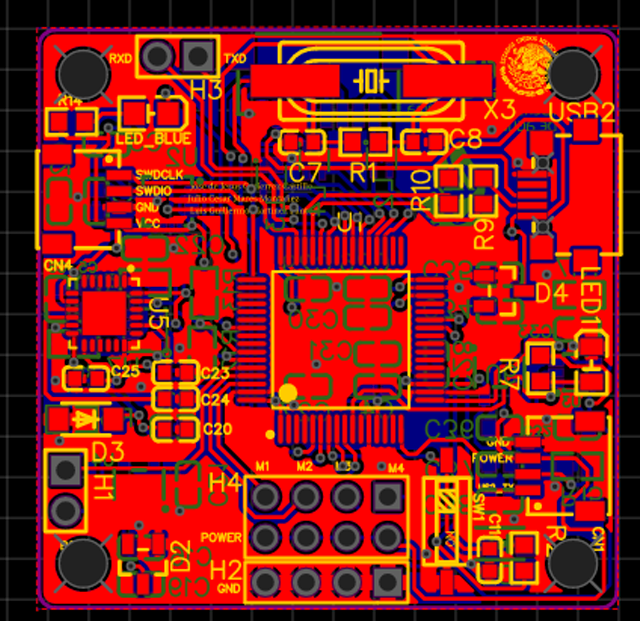
\includegraphics[width=0.5\linewidth]{src/PCB.png}
    \caption{ PCB del diseño de la FC}
    \label{fig:placeholder}
\end{figure}

Una vez realizado el diseño del PCB se mandó a hacer con la página “JLCPCB”, y el resultado es el 

\begin{figure}
    \centering
    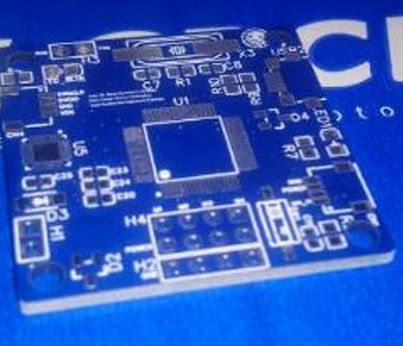
\includegraphics[width=0.5\linewidth]{src/PCB Fisico.png}
    \caption{PCB Fisico de la FC}
    \label{fig:placeholder}
\end{figure}

Al ver todos los precios del PCB, los componentes para soldar, nos dimos cuenta de que la controladora 
de vuelo resultaría más costosa que comprar una ya construida, por lo que se optó por no continuar 
con la construcción de esta FC, y menos con la programación, ya que no tiene caso, ya que el código 
sería muy similar al que una CC3D tiene. Pero si se quiere mejorar este diseño tanto en componentes o con programación, en el apartado “Control”, viene una breve explicación de cómo se debe hacer el 
control para los motores de un drone.

\subsubsection{Control}

Para el control tenemos a la planta, la cual sería el drone en sí, también tenemos 4 actuadores que serían los motores que inyectan fuerzas y torques al sistema, la salida del sistema serían las variables tomadas de los sensores, estos sensores son la unidad de medición inercial que es el acelerómetro, este cuenta con 6 ejes, 3 del acelerómetro y otros 3 del giroscopio, también tenemos un barómetro el cual mide la altura a la que está el sistema mediante la presión del aire. Como entrada tenemos al punto de referencia, 
este nos indica que es lo que queremos que haga el drone, también tenemos un controlador el cual se va a encargar de tomar todos estos datos de salida y de entrada y de esta manera controlar a los motores mediante un algoritmo, el diagrama de bloques del control mencionado se muestra a continuación: 
 
\begin{figure}[!h]
    \centering
    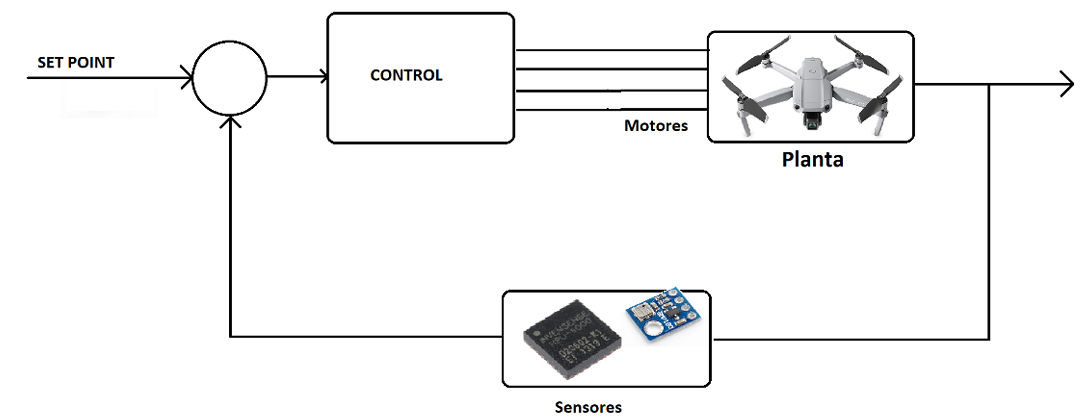
\includegraphics[width=0.5\linewidth]{src/Bloques.png}
    \caption{Esbozo del control para un drone.}
    \label{fig:placeholder}
\end{figure}
Ahora hablemos de los movimientos del drone. Las direcciones de traslación del drone son: arriba y abajo, izquierda y derecha, y atrás y adelante. Las direcciones rotacionales son: roll, pitch y yaw (alabeo, cabeceo y guiñada).


\begin{figure}[!h]
    \centering
    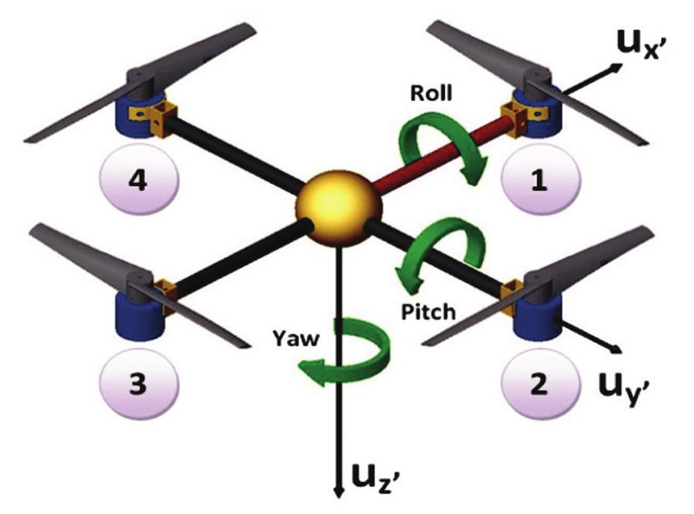
\includegraphics[width=0.5\linewidth]{src/Movimientos de un drone.png}
    \caption{Movimientos de un dron}
    \label{fig:placeholder}
\end{figure}
Para lograr todos estos movimientos contamos con únicamente 4 motores, tenemos 6 grados de libertad por lo que estamos delante de un sistema sub actuado.

Un motor se eleva gracias a hacer girar a la propela la cual impulsa aire hacia abajo causando una fuerza de reacción que va hacia arriba. Si el motor está colocado de forma que la fuerza aplicada esté en el centro de gravedad de un objeto, entonces este objeto se moverá en traslación pura sin rotaciones.

\begin{figure}[!h]
    \centering
    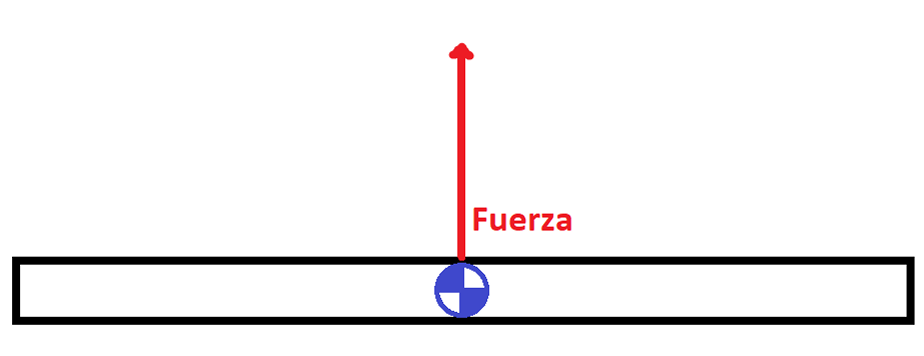
\includegraphics[width=0.5\linewidth]{src/Objetosometidoafuerza.png}
    \caption{Objeto sometido a fuerza}
    \label{fig:placeholder}
\end{figure}
Otra cosa a destacar es que si la fuerza producida por el motor es igual a la fuerza de gravedad entonces el objeto se mantendrá en el mismo lugar.

Una fuerza a una distancia del centro de gravedad produce tanto movimientos traslacionales como movimiento rotacional con referencia del centro de gravedad.

Para contrarrestar el torque de reacción, podemos hacer que ambos motores giren en direcciones contrarias. De esta manera funciona bien para dos dimensiones pero el sistema no sería capaz de generar torques en 3 dimensiones por lo tanto agregaremos una segunda barra con otros dos motores lo que creará a nuestro cuadricóptero.

Con esta configuración podemos mantener estable a nuestro drone acelerando cada uno de los motores hasta que cada uno produzca 1/4 de la fuerza de gravedad. Ya que tenemos dos motores girando en dirección contraria, los torques de giro producidos por las propelas se balancearán y el drone no girará.

Si queremos hacer el movimiento de yaw debemos disminuir la velocidad de los dos motores que giran en una misma dirección y aumentar la velocidad de los otros dos.

Para hacer el movimiento de roll debemos decrementar la velocidad de uno de los pares de motores ya sea de izquierda o de derecha e incrementar el otro par.

Para hacer el movimiento de pitch debemos decrementar uno de los pares de motores ya sea de enfrente o detrás e incrementar el otro par.

Este es nuestro simple algoritmo llamado ``motor mixing algorithm'' el cual se muestra en forma de ecuaciones a continuación:

$$\begin{aligned}
\text{Motor}_{\text{frente\_derecha}} &= \text{Elevación} + \text{Yaw} + \text{Pitch} + \text{Roll} \\
\text{Motor}_{\text{frente\_izquierda}} &= \text{Elevación} - \text{Yaw} + \text{Pitch} - \text{Roll} \\
\text{Motor}_{\text{atrás\_derecha}} &= \text{Elevación} - \text{Yaw} - \text{Pitch} + \text{Roll} \\
\text{Motor}_{\text{atrás\_izquierda}} &= \text{Elevación} + \text{Yaw} - \text{Pitch} - \text{Roll}
\end{aligned}$$

Para mover a nuestra disposición al drone contamos con un control remoto, este cuenta con principalmente dos palancas que se pueden mover hacia arriba y hacia abajo y a la izquierda y derecha. En la primer palanca (la de la izquierda) al moverla hacia arriba y hacia abajo podemos cambiar la elevación de nuestro drone, y al moverlo hacia la izquierda o la derecha cambiamos el ángulo de yaw. La palanca de la derecha sirve para cambiar el pitch y el roll de nuestro drone.

Para comenzar diseñaremos un control en el que se utilice la variable de elevación para controlar la altitud a la que está el drone. Si somos capaces de medir la altura a la que está el drone entonces podemos tomar ese valor y compararlo con el valor que queremos. El error resultante alimentará a nuestro control el cual utilizará esta información para determinar si incrementar o decrementar la velocidad de los motores. Por ahora podemos pensar en este control como un PID.

De esta manera si nuestro drone está volando muy bajo y nuestra referencia está en un punto más alto entonces el error será positivo comandando a los 4 motores a incrementar la velocidad al mismo tiempo. Si nuestro drone está volando más alto que nuestra referencia entonces el error será negativo comandando a nuestros 4 motores para disminuir la velocidad.

En la vida real hay perturbaciones como por ejemplo las corrientes de aire las cuales van a inducir movimientos de pitch o de roll a nuestro sistema. De esta manera tenemos que diseñar un control que sea capaz de controlar todos los movimientos, ya sea de yaw, pitch y roll independientemente sin afectar a los demás. Podemos crear otros 3 controles PID de yaw, pitch y roll exactamente de la misma manera que hicimos con la elevación.

Ahora solo tenemos que hacer la difícil tarea de sintonizar cada uno de los controladores PID, afortunadamente para nosotros, las controladoras de vuelo ya tienen un programa que hace este proceso.

\subsection{Construcción}

Primero se hizo una estimación del peso que iba a tener el drone, contando con el peso de módulos, motores y la carcasa. Entonces lo que se debe hacer primero es seleccionar una carcasa. Al ver en las comparaciones de carcasa, se selecciona una que dependiendo del drone sea la más adecuada. Por ejemplo, si es un drone de carreras lo ideal sería escoger una pequeña, que no pese mucho.

Después de seleccionar la carcasa, se debe seleccionar la batería. Se debe tener cuidado al seleccionar esta parte, ya que los módulos como la CC3D o controladora de vuelo, el distribuidor de energía, las ESC, dependen de un voltaje en específico. Recomendamos comprar una batería con 11.1 V de salida o 3s de celdas.

Teniendo en cuenta la batería, se seleccionó el distribuidor de energía y los ESC. Comúnmente los ESC no tienen muchas diferencias entre ellos, por lo que se deben seleccionar unos que brinden un peso bajo y un amperaje alto contra el precio de este.

Luego se seleccionó la parte más importante del drone, la cual es la controladora de vuelo. Se seleccionó la CC3D, este es un controlador de vuelo potente y asequible que es muy popular para usar principalmente en helicópteros miniquad.

Contando ya con todos las partes del drone y con la investigación llevada a cabo de los motores, se realizó una selección de un motor. Se hizo una estimación del peso que tendría el drone y dependiendo del empuje del motor y del precio se seleccionaron unos en concreto.

Entonces contando con todos los elementos se realizó la construcción del drone.

\subsection{Conexiones del Sistema}

Para el receptor tenemos 3 filas de pines, la primera corresponde a la señal de PWM (S) de cada canal, la segunda y tercera corresponden a VDD y GND respectivamente.

El receptor se conectará directamente a la controladora de vuelo por medio de un conector JST. El conector debe conectarse de manera que el conector 1, el cual tiene 3 cables (rojo para VDD, negro para GND, y blanco para S), esté en el CH1 del receptor, y así en orden para todos los demás conectores.

Lo siguiente es soldar los ESC al PDB, y los ESC a cada uno de los motores. En la fila 1 del conector conectaremos al ESC que controla al motor 1, en la fila 2 conectaremos al ESC que controla al motor 2, y así con todos los demás.

\subsection{Calibración de la controladora de vuelo con LibrePilot}

La calibración se va a realizar mediante el software libre ``LibrePilot''. Para calibrarlo seleccionaremos la opción ``Vehicle Setup Wizard''.

A continuación, nos mostrará una ventana, la cual nos actualizará nuestra controladora de vuelo.

Después aparecerá una ventana, en la cual seleccionaremos el método de comunicación PWM.

Luego, seleccionaremos la opción ``Multirotor'', la cual nos indicará cómo deberán girar los motores del drone.

En la siguiente ventana seleccionaremos la opción ``Rapid ESC''.

Después de las configuraciones anteriores, nos mostrará una ventana con un resumen de todo lo que hemos seleccionado y daremos en next. Lo siguiente será calibrarlo, por lo que el drone deberá estar en una superficie plana.

Luego sincronizaremos nuestros ESC para que puedan regular la velocidad de los motores, para esto seguiremos todas las instrucciones que nos aparecen en la ventana.

Después de esto calibraremos el valor mínimo de voltaje que necesitan los motores para comenzar a girar, para esto necesitaremos mover la barra hasta que comience a girar el motor, este proceso se repite con cada uno de los motores.

Luego seleccionaremos un modelo para nuestro drone, cuidando que las características sean parecidas al nuestro y guardaremos las configuraciones.

Después seleccionaremos el modo de nuestro control en el modo ``Acro''.

Por último, seleccionaremos la configuración de los joysticks en modo 2.

Por último, seguiremos las instrucciones que nos aparecerán en la pantalla y terminaremos la calibración.

\section{Resultados}

El drone fue construido exitosamente y se pudo calibrar y probar en vuelos. Un video del drone funcionando se puede ver en el siguiente enlace:

\begin{center}
\url{https://youtu.be/-E99j_d1kX4}
\end{center}


\begin{thebibliography}{99}

\bibitem{OscarLiang1}
Oscar Liang (2024) \textit{Flight Controller}
Recuperado de \url{https://oscarliang.com/flight-controller/}

\bibitem{oscarlipo}
Oscar Liang (2024) \textit{Lipo battery guide}
Recuperado de \url{https://oscarliang.com/lipo-battery-guide/
}


\bibitem{stm32ventajas}
Ampheo (2025) \textit{Which microcontrollers are used in drones?}
Recuperado de \url{https://www.ampheo.com/blog/which-microcontrollers-are-used-in-drones?srsltid=AfmBOorKWpPFcAOCYTDtfuYw_VUTffBz84NHnF7gj-R52XHiEEHEF7zX}

\bibitem{rogerlipo}
Brian Schneider  (2021) \textit{A Guide to Understanding LiPo Batteries} 
Recuperado de \url{https://www.rogershobbycenter.com/lipoguide}
% https://www.youtube.com/watch?v=DeSDjjicGWY
 

\bibitem{gensacelipo}
Tattu Gens Sace  (2024) \textit{LiPo Battery Guide} 
Recueperado de https://gensace.de/pages/lipo-battery-guide


\bibitem{rclipo}
Guides d'achat  (2025) \textit{The LiPo Battery Guide} 
Recueperado de https://www.rcteam.com/en/blogs/the-rc-model-blog/lipo-battery-guide

\end{thebibliography}

\end{document}
